\section{Experimental Results}

We have implemented Garg-MCF in the Python programming language and tested it
upon a variety of input problems using the PyPy JIT compiler. Due to the
automatic garbage collection and high level nature of Python, the clock time of
our implementation should be taken with a grain of salt. We report the number
of calls to the single-source shortest path subroutine as a more reliable
performance indicator, as we make one call per phase of the algorithm. We first
describe the construction of random graphs.

We construct random directed graphs using the networkx module's
$\mathrm{gnm\_random\_graph}$ routine, feeding parameters of $n$ and $m$
\cite{networkx}. Then we randomly create commodities by a grouping procedure.
We take the number of commodities as a parameter and a distribution which
defines the number of shared source commodities we have, randomly choosing
sinks for the commodities, ensuring that there exists a directed path from the
source to the sink for each commodity. Capacities and demands are chosen at
random. This set of procedures allows us to randomly generate a directed graph
with a given number of nodes, edges, commodities, and we can explicitly specify
the number of commodity groups. With this in hand, we can proceed to test the
algorithm's dependence on parameters \{$\omega$, $k$, $n$\}, taking note of the
effect of Karakostas' heuristic for shared source commodities.

We initially validated the correctness of our algorithms by running on several
small graphs $(m<\leq 10)$ with multiple commodities that could be optimized by
hand. Included in these test cases were multiple commodities with shared and
unshared sources, and demands that vary orders of magnitudes to empirically
validate relaxation on demand-scaling. We found our implementation provided an
answer within the $(1+\omega)$ approximation ratio on all test cases and thus
proceed confidently with the following experiments.

\subsection{Dependence on the parameter $\omega$}

\begin{figure*}\begin{center}\mbox{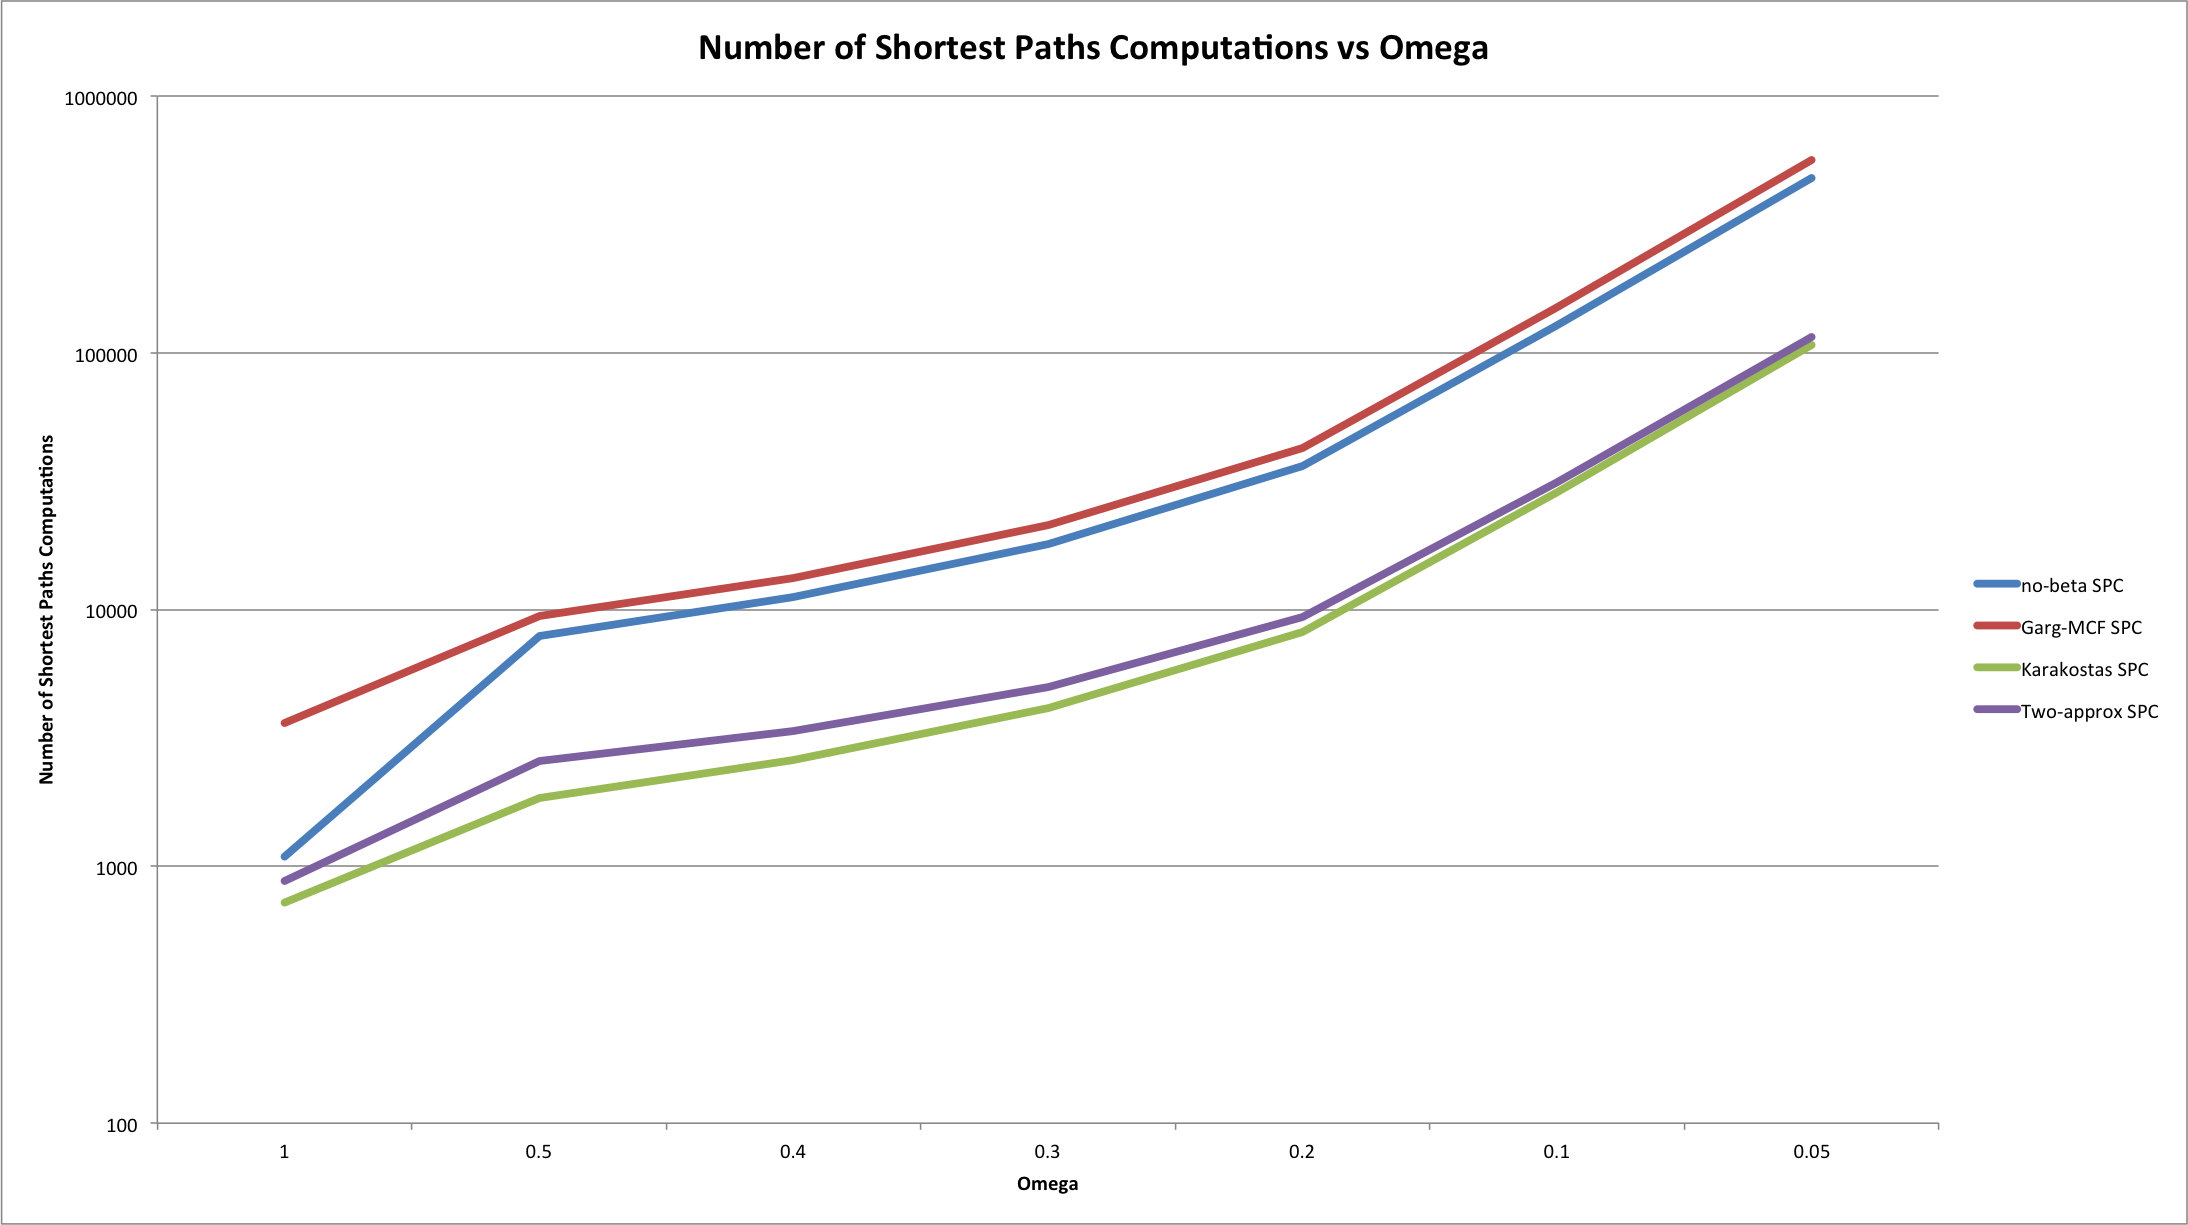
\includegraphics[width=0.8\textwidth]{figures/omegas.png}}
\caption{Plots of number of shortest-path computations versus error term
$\omega$ for all heuristics. This data was obtained from running our
algorithm, with the respective heuristics activated, on graphs with $100$
nodes, $400$ directed edges, 10 commodities (split into two groups of size 6
and 4 that shared the same source) on 10 different random graphs. Of the 10
measured shortest path computations for each $\omega$, we dropped the minimum
and maximum, and reported the average over the remaining.} \end{center}
\end{figure*}
In theory, the Garg-MCE algorithm runs
with a quadratic dependence on $\omega$, which we observe in practice, both in
terms of number of calls to our shortest paths function, and also wall time.


We observe that the algorithm works correctly and even slightly more
efficiently if we do \emph{not} scale $\beta$ such that it is bounded above by
1, as previous analysis assumes.

The two-approximation heuristic was implemented on top of Karakostas' heuristic
and we do not observe it outperforming just Karakostas' heuristics. However,
our data hints that the two-approximation may be asymptotically more optimal,
but, regrettably, limited precision arithmetic on primitive floats and
expensive computations on arbitrary precision decimals render testing smaller
values of $\omega$ infeasible.

We include data on physical time performance in the appendix.

\subsection{Dependence on the parameter $k$} \begin{figure*} \begin{center}
\mbox{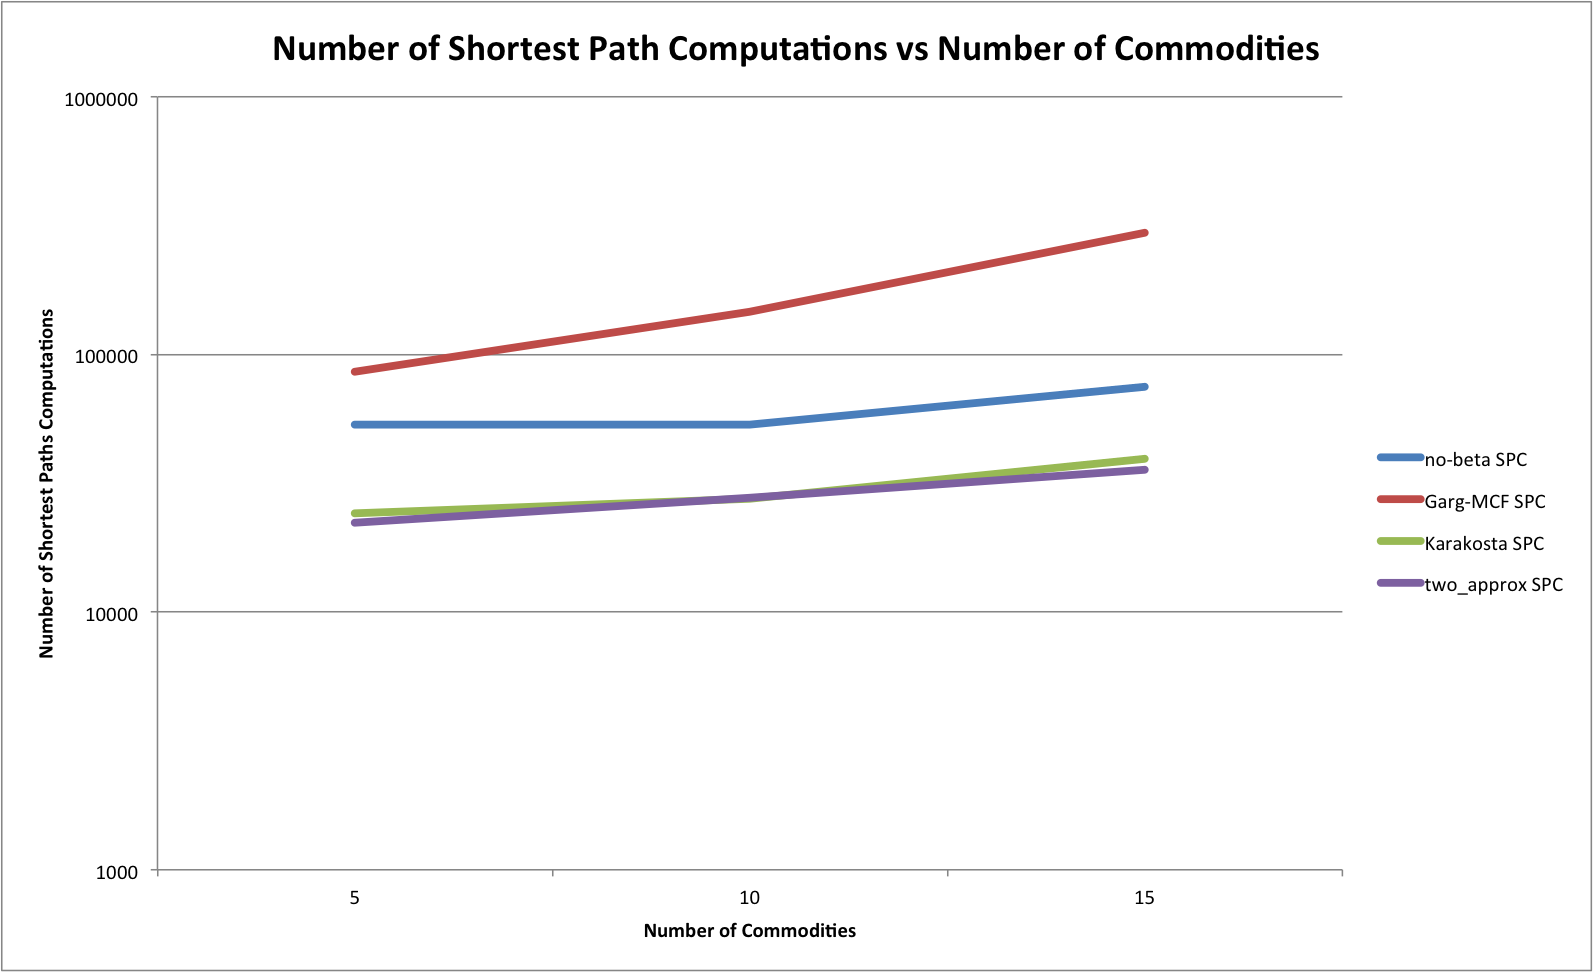
\includegraphics[width=0.8\textwidth]{figures/commodities.png}}
\caption{Plots of number of shortest-path computations versus number of
commodities $k$ for all heuristics. This data was obtained from running our
algorithm, with the respective heuristics activated, on graphs with $100$
nodes, $400$ directed edges, and a error margin of $10\%$, 10 times.  }
\end{center} \end{figure*}

The Garg-MCE algorithm has a linear dependence on k, and the Karakostas
heuristic absorbs this factor.

Again, we observe our vanilla implementation outperforming the implementation
with $\beta$ scaling, the Karakostas heuristic outperforming both, and the
two-approximation having similar performance.

\subsection{Dependence on the parameter $n$} \begin{figure*} \begin{center}
\mbox{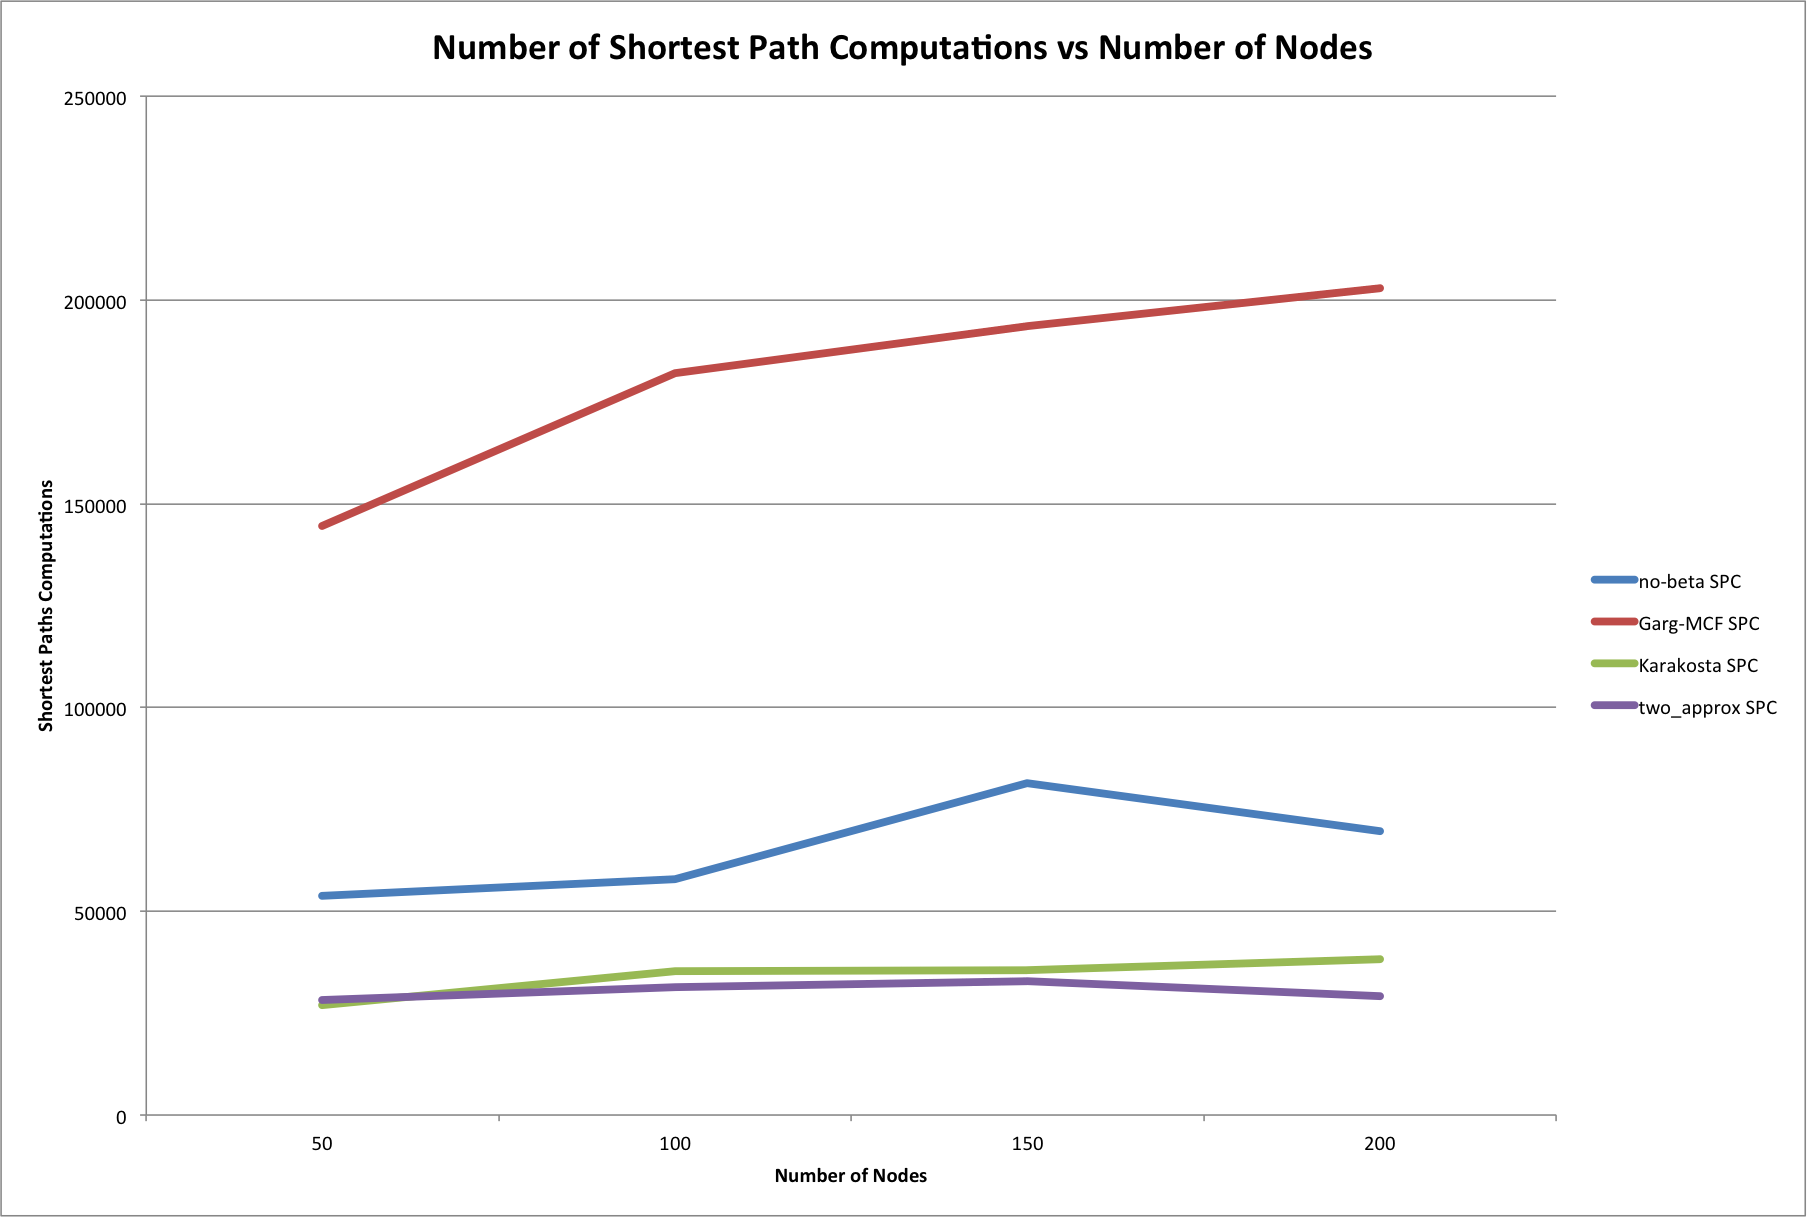
\includegraphics[width=0.8\textwidth]{figures/nodes.png}} \caption{Plots
of number of shortest-path computations versus number of nodes for all
heuristics. This data was obtained from running our algorithm, with the
respective heuristics activated, 10 commodities (split into two groups of size
6 and 4 that shared the same source), and an error margin of $10\%$, 10 times.
We construct our graphs such that the number of edges is always four times the
number of nodes. } \end{center} \end{figure*}

Our algorithm has a quadratic dependence on the number of edges, comparable to
the number of nodes, given our sparse graph.  We expect and observe there to be
a linear dependence of the number of shortest path calls on the number of
nodes.

A surprising result is that this dependence is experimentally not very strong
for relatively small $n$: we observe that the number of calls to shortest paths
does not necessarily increase with an increase in graph size.

\subsection{Dependence on the distribution}

\begin{figure*} \begin{center}
\mbox{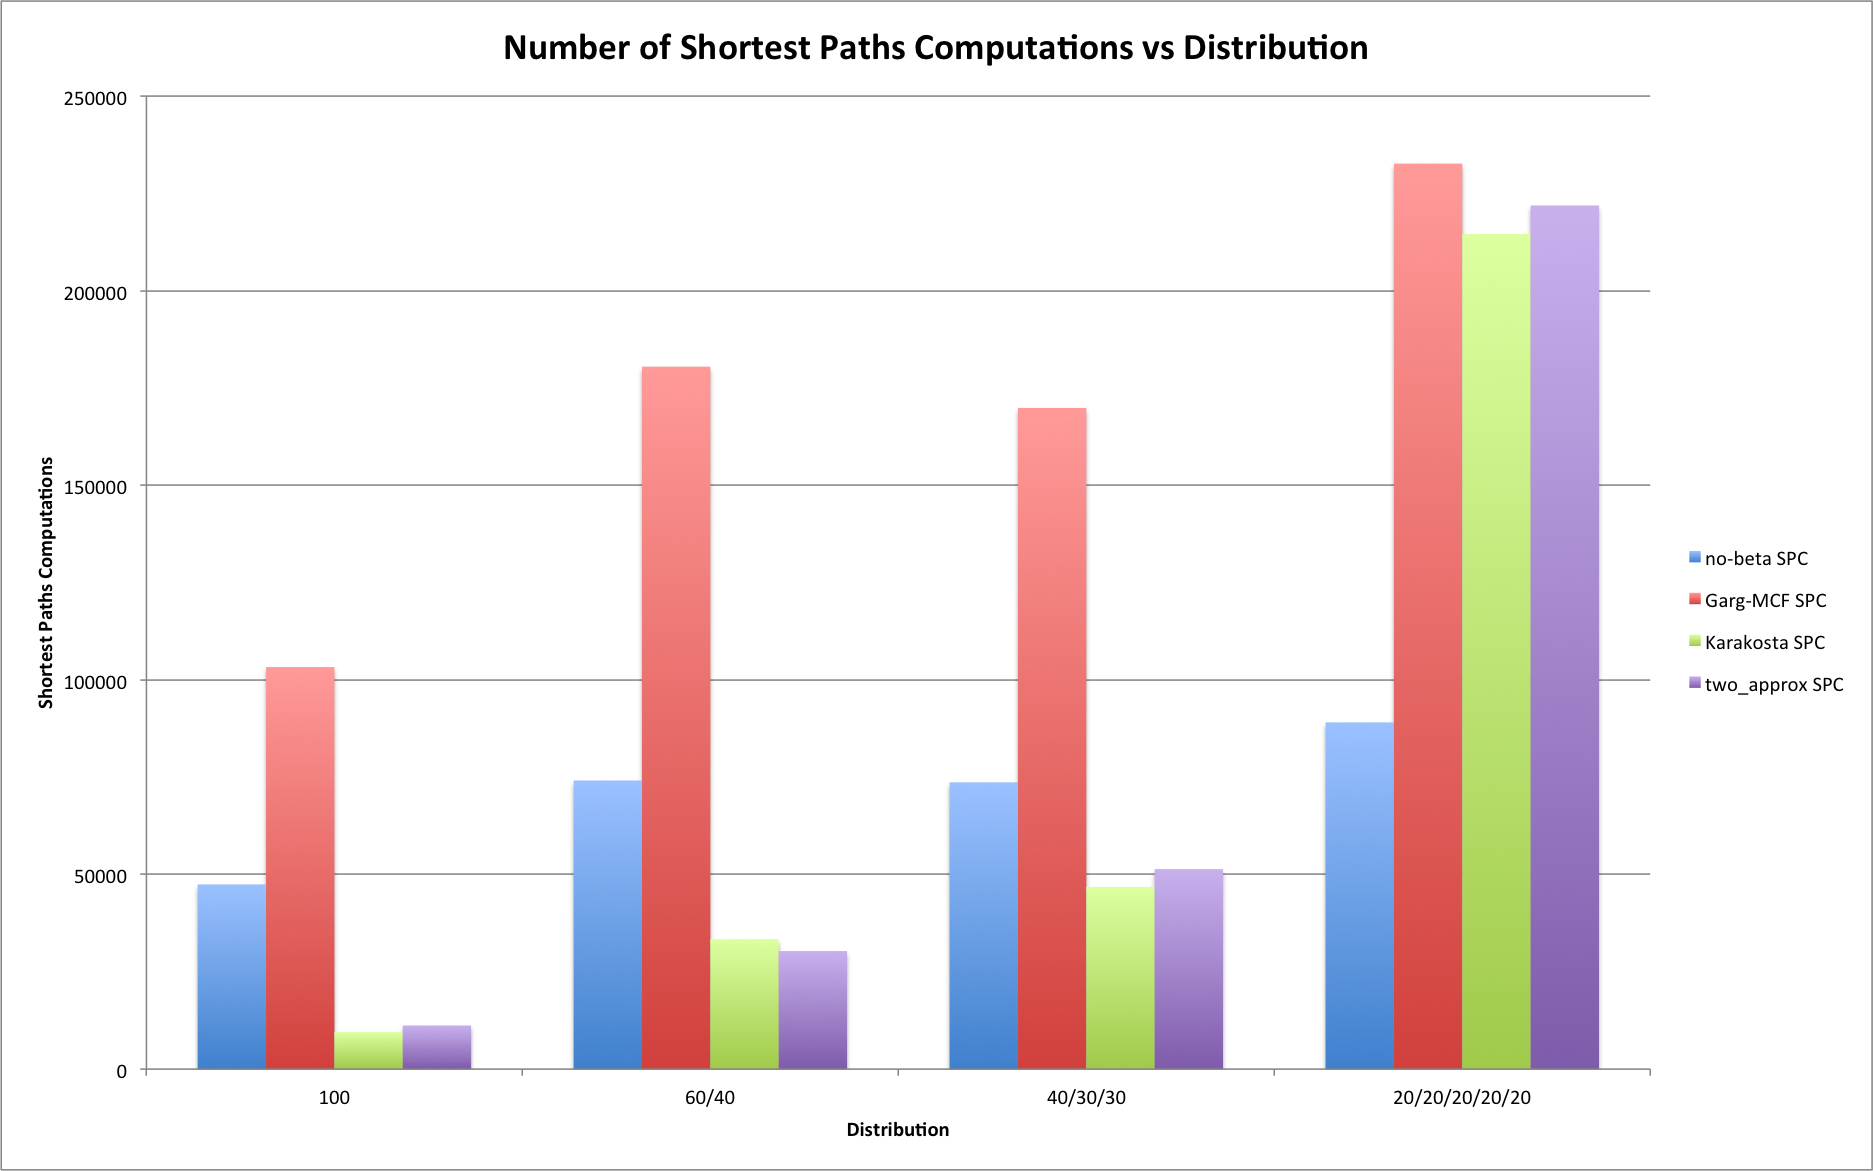
\includegraphics[width=0.8\textwidth]{figures/distribution.png}}
\caption{Plots of number of shortest-path computations versus number of nodes
for all heuristics.This data was obtained from running our algorithm, with the
respective heuristics activated, on graphs with $100$ nodes, $400$ directed
edges, 10 commodities, 10 times. Each time, we vary the distribution of
commodities that share the same source.} \end{center} \end{figure*}

Our algorithm does not strictly depend on how the commodities are distributed,
but the Karakostas heuristic takes advantage of multiple commodities that start
at the same source. We expect the Karakostas heuristic to significantly
outperform baseline in the case where all the commodities start at the same
source, and underperform when all the commodities start at differing sources.

Somewhat surprisingly, our baseline vanilla and beta algorithms are dependent
on the input distribution.  We hypothesize that this may be due to underlying
caching optimizations that work more efficiently when the search algorithm is
more predictable and visits the same nodes initially.

